\documentclass[twoside]{article}

% Use the attached latex template to write the proposal for your final project. The page limit of the proposal is 2 pages. Project proposals must be different than (or at least a significant extension of) projects submitted for STA 561. Project proposal grades will be factored in to the final project portion of this course. All proposals must be submitted by March 17th.

\usepackage{epsfig}
\usepackage{hyperref}

\setlength{\oddsidemargin}{0.25 in}
\setlength{\evensidemargin}{-0.25 in}
\setlength{\topmargin}{-0.6 in}
\setlength{\textwidth}{6.5 in}
\setlength{\textheight}{8.5 in}
\setlength{\headsep}{0.75 in}
\setlength{\parindent}{0 in}
\setlength{\parskip}{0.1 in}

\newcommand{\lecture}[4]{
   \pagestyle{myheadings}
   \thispagestyle{plain}
   \newpage
   \setcounter{page}{1}
   \noindent
   \begin{center}
   \framebox{
      \vbox{\vspace{2mm}
    \hbox to 6.28in { {\bf STA571:~Advanced machine learning \hfill} }
       \vspace{6mm}
       \hbox to 6.28in { {\Large \hfill #1 (#2)  \hfill} }
       \vspace{6mm}
       \hbox to 6.28in { {\it Authors: #3} \hfill}
      \vspace{2mm}}
   }
   \end{center}
   \markboth{#1}{#1}
   \vspace*{4mm}
}

\begin{document}

\lecture{Classifying Olympic Athletes by Sport}{\today}{Matt Dickenson}

% keep this document to one page.

\section{Motivation}

%What is the real-world problem your project will address? What data
%will motivate your methodology?  

To what extent do environmental or biological traits determine sporting success? At the highest level of amateur sports--the Olympic games--we can notice differences in the physical characteristics of participating athletes across sports. For example, the median height for male participants in the 2012 games was 182 centimeters, but the median male basketball player was 202cm while half of male gymnasts were shorter than 167cm. Similar disparities exist in weight and age. 

Can these differences be exploited to classify individuals by sport or event given their physical attributes? If this could be done with a high degree of accuracy, that would suggest that athletes are increasingly optimizing for success by selecting sports for which they are naturally predisposed. If not, we could infer that training makes more of a difference than genetically determined features. To study this question, I will use data on participants in the 2012 Summer Olympic Games published by \href{http://www.theguardian.com/sport/datablog/2012/aug/07/olympics-2012-athletes-age-weight-height#data}{\emph{The Guardian}}. 
% todo: cite David Epstein here


\section{Problem definition} 

%Define this problem quantitatively. What question are you trying to
%solve? What are the random variables? What is the goal of the project?

% todo: make this notation match the stuff below
The goal of this project is to predict an athlete's Olympic event given their height, weight, age, and gender. Given data $\mathcal{D}$ on these $p=4$ features for $n=9,038$ athletes,\footnote{There were 10,383 participants in the 2012 games. The 9,038 figure accounts for missingness on the feature variables.} our goal is to predict of athletes' events $\mathbf{y}$, which are nested in sports.\footnote{In the Olympic games, ``sports'' are somewhat broad categories, such as athletics and weightlifting, whereas ``events'' refers to specific competitions such as the men's 100-meter race.} The quantity we are interested in, then, is $p(\mathbf{y}|\mathcal{D})$.

Figure \ref{bball-weight} displays the height, weight, and sex of 487 participants (258 basketball players and 229 weightlifters). Although not all clusters are as distinct as these, this does suggest that clustering methods could accurately classify Olympic athletes by event.

\begin{figure}
\begin{center}
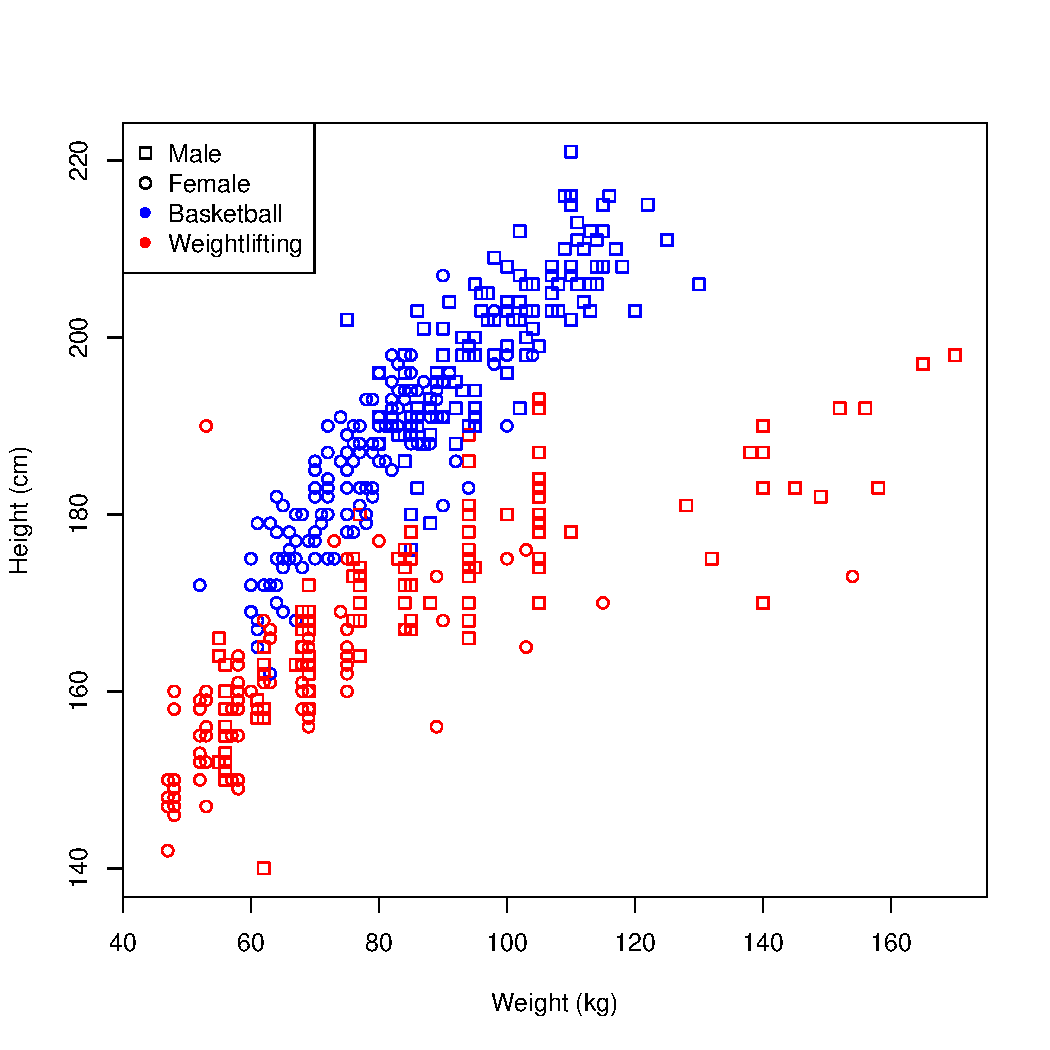
\includegraphics[scale=0.5]{./project/Basketball-Weightlifting.pdf}
\caption{2012 Olympic Participants in Basketball and Weightlifting, by Height and Weight}
\label{bball-weight}
\end{center}
\end{figure}

\section{Models and methods}

%What probabilistic approach will you take to solve the problems? What
%parameters will be estimated, and how will you estimate those
%parameters? Do the parameters have interpretations in terms of the
%solution to the problem you are trying to answer?

% todo: cite Heller here
To classify athletes by event, this project will employ Bayesian hierarchical clustering (BHC). BHC models will be trained on subsets of the data using $k$-fold cross-validation with (randomly sampled) training sets of $10,20,\ldots,90$ percent of the original dataset. This method is sensible for Olympic athlete data because participants in two different events within the same sport category should be more similar than those in different sports. For example, we can discover whether an athlete running the 100m event has more in common with a 5000m runner (both distances are classified under ``Athletics'') or a volleyball player.

In order to classify an athlete from the test set, we can use the posterior predictive distribution
\begin{eqnarray*}
p(\mathbf{y}|\mathcal{D}) &=& \sum_{k \in N} w_k p(\mathbf{y}|\mathcal{D}_k),
\end{eqnarray*}
where $w_k$ is the weight on cluster $k$, $\mathcal{D}_k$ is the feature data for observations in cluster $k$, $N$ is the set of nodes in the tree, and $N_k$ represents the nodes lying on the path from the root to node $k$'s parent. 

\section{Results and validation}

% What will your results show? How will you quantify how well this 
% approach answered the question? What other models/methods will you 
% compare these results against? How will you validate the answers 
% and your uncertainty in the answers?

The results of this method will be compared to classification with a multinomial GLM and CART. To assess these methods, we will use classification accuracy as measured in the cross-validated models (this is necessary because a single run of BHC or CART does not express uncertainty in the classifications). BHC should do well because it relies on comparing marginal likelihoods of subtrees for merging, rather than distance metrics.

In substantive terms, these results will show whether an athlete's event can be accurately predicted by their physical features. If not, that would suggest that athletic ability can be understood as a latent trait that can be applied to the sport of one's choice. If the model can accurately predict participation in an event using the features specified, that suggests that athletes choose the event that best leverages their natural predisposition. The answer to this question will be important we ponder the future of athletic performance.

% do not include references in this document; your final document will be
% allowed unlimited citations.

\end{document}
